\documentclass{article}
\usepackage{tikz}
\usepackage{circuitikz}
\usepackage{amsmath}
\usepackage{cleveref}
\usepackage[a4paper]{geometry}
\crefname{equation}{}{}
\Crefname{equation}{}{}

\begin{document}
A DC motor drives a mechanical load.
The task is to follow some reference speed profile, while providing the required load torque.
This load torque is regarded as an unknown, unmeasured disturbance.
The DC motor uses one of two electrical drives for control purposes.

\section{Load}
The time-variable load torque $T_u(t)$ represents the useful mechanical work being done (for example in an elevator, the work needed to move the elevator cage).
For this demo it is assumed to uncontrollable and independent of the rotational speed of the motor.
The mechanical drive is modelled as a rotational mass-damper system with Coulomb friction.
The total torque at the motor shaft is given by \cref{eq:loadtorque,eq:coulombtorque} where $J$ is the moment of inertia, $B$ the damper constant and $\tau_{coulomb}$ the friction constant.

\begin{align}
  T_l &= J\frac{d\omega}{dt} + B \omega + T_{coulomb}(\omega) + T_{u}(t) \label{eq:loadtorque}\\
  T_{coulomb}(\omega) &= \begin{cases}
    \tau_{coulomb} & \omega > 0\\
    0 & \omega = 0\\
    -\tau_{coulomb} & \omega < 0
  \end{cases} \label{eq:coulombtorque}
\end{align}


\section{DC Motor}
The motor armature is represented by \cref{fig:motor}.
The rotation of the motor armature in the magnetic field causes a back-EMF $e$ to be induced \cref{eq:emf}, where $C$ is a motor constant, $\omega$ is the angular velocity and $\phi$ is the magnetic flux induced by the excitation windings.
Likewise, the motor torque $T_m$ is given by \cref{eq:motortorque}.
The magnetic flux is directly proportional to the excitation current $i_b$, such that both equations can be rewritten as \cref{eq:emfib,eq:motortorqueib} with $k$ some motor constant.
Circuit analysis on \cref{fig:motor} allows to derive \cref{eq:armaturecircuit}.
Note that DC machines can work in both motor and generator regime: here we use the convention that if $i_a > 0$ the machine works as a motor (e.g. it drives the mechanical load).
Finally, consider that the torque at the motor shaft as defined in \cref{eq:loadtorque} must be equal to the generated torque \cref{eq:torquebalance}.
\begin{figure}
  \centering
  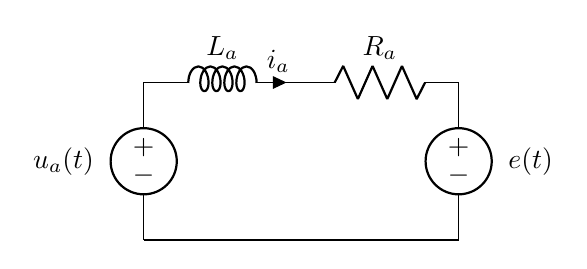
\begin{tikzpicture}[american voltages]
    \draw (0, 0) to [V=$u_a(t)$, invert] (0, 2) to [L=$L_a$, i=$i_a$] (2, 2) to [R = $R_a$] (4, 2) to [V=$e(t)$] (4, 0) to[short] (0, 0);
  \end{tikzpicture}
  \caption{Equivalent circuit of the motor armature}
  \label{fig:motor}
\end{figure}

\begin{align}
  e &= C \dot{\theta}\phi \label{eq:emf}\\
  T_m &= C i_a \phi \label{eq:motortorque}\\
  e &= k \omega i_b \label{eq:emfib}\\
  T_m &= k i_ai_b \label{eq:motortorqueib}\\
  u_a &= e + R_a i_a + L_a \frac{di_a}{dt} \label{eq:armaturecircuit}\\
  T_m &= T_l \label{eq:torquebalance}
\end{align}

The excitation winding (\cref{fig:excitation}) has inductance $L_b$ and parasitic resistance $R_b$. The equation \cref{eq:excitation} relating the excitation current $i_b$ and voltage $u_b$ follows from trivial circuit analysis.
\begin{align}
  u_b = L\frac{di_b}{dt} + Ri_b \label{eq:excitation}
\end{align}

\begin{figure}
  \centering
  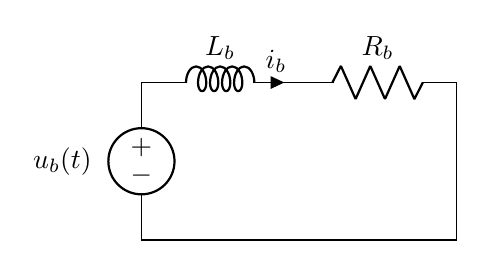
\begin{tikzpicture}[american voltages]
    \draw (0, 0) to [V=$u_b(t)$, invert] (0, 2) to [L=$L_b$, i=$i_b$] (2, 2) to [R = $R_b$] (4, 2) to[short] (4, 0) to[short] (0, 0);
  \end{tikzpicture}
  \caption{Equivalent circuit of the motor excitation windings}
  \label{fig:excitation}
\end{figure}
\section{Electrical Drive}
The electrical drive aims to follow an angular velocity profile $\omega_{ref}(t)$ by regulating the voltages $u_a$ and $u_b$.
It has access to a perfect, noise-free measurement of $\omega$.
The drive operates in one of two modes:
\begin{enumerate}
  \item Separate connection of excitation and armature windings. In this mode, a fixed excitation current is used and the control is done by varying $u_a$.
  \item Parallel connection of excitation and armature windings. In this mode, $u_a = u_b$ at all times.
  \end{enumerate}
A PI controller with parameters $K_i$ and $K_p$ is used to set the voltage output \cref{eq:control}.
For simplicity we assume that the electrical drive can provide an arbitrarily large voltage and that the DC motor can withstand such voltages (i.e. no saturation).
\begin{align}
  u_a &= K_i \int_0^t (\omega_{ref} - \omega) dt + K_p (\omega_{ref} - \omega) \label{eq:control}
  \end{align}

\section{Summary}
For ease of implementation, the full system of equations is transformed into an ODE in \cref{eq:summary}.
We introduce the variable $c(t)$ which represents the state of the integrator in the PI controller.

\begin{subequations}
  \label{eq:summary}
\begin{align}
  J\frac{d\omega}{dt} &= -B\omega - T_{coulomb}(\omega) - T_u(t) + k i_a i_b  \\
  L_a\frac{di_a}{dt} &= \left(K_i c + K_p (\omega_{ref}(t) - \omega)\right) ki_b\omega - R_a i_a     \\
  L_b\frac{di_b}{dt} &= u_b - Ri_b  \\
  K_i \frac{c}{dt} &= (\omega_{ref}(t)-\omega)
\end{align}
\end{subequations}
\end{document}
